\documentclass[letterpaper, 12pt, final]{report}

\linespread{1.5}

\usepackage{hyperref}
\hypersetup
{
    pdftitle = {Curriculum Vitae de Madelin Díaz Ramos},
    pdfauthor={\textcopyright\ Madelin Díaz Ramos},
    pdfsubject={Curriculum Vitae de Madelin Díaz Ramos},
    pdfkeywords={Curriculum Vitae, Madelin Díaz Ramos},
    pdfpagemode={UseOutlines},
    bookmarksopen,
    pdfstartview={FitH},
    colorlinks,
    linkcolor={blue},
    citecolor={green},
    urlcolor={blue}
}

%------language packages----------------

\usepackage[utf8]{inputenc}
\usepackage[spanish, activeacute, es-tabla]{babel} %for documents in spanish

%----------image packages---------------

\usepackage{graphicx}
\usepackage{subfigure}

%------enumerating packages-------------

\usepackage{enumitem}


%----------page layout------------------

\oddsidemargin 0.36cm
\evensidemargin 0.36cm
\marginparwidth 0.0cm
\textwidth 15.80cm

\topmargin -1.5cm
\headheight 1.0cm
\headsep 1.0cm
\footskip 1.0cm
\textheight 21.34cm

\hyphenation {cuba}
\hyphenation {universidad}
\hyphenation {functional}
\hyphenation {matematica}

%----------document start---------------

\begin{document}

\begin{center}
	\textbf{Curriculum Vitae - Madelin Díaz Ramos}
\end{center}

\vskip 0.5cm

%% my picture
%\begin{figure}[h]
%	\centering
%	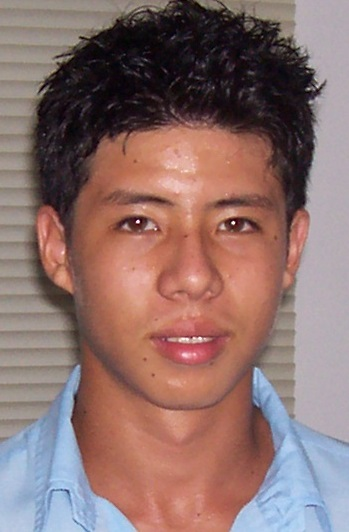
\includegraphics[scale=0.3]{images/cv-02.jpg}
%	\label{fig:presentation-picture}
%\end{figure}
%
%\vskip 1cm

%----------------------------------------------------------------------------------

\underline{\textbf{Información Personal:}}

\begin{itemize}[noitemsep, nolistsep]
	
	\item Nombre: Madelin Díaz Ramos.
	\item Nacionalidad: Cubana.
	\item Fecha de Nacimiento: 28 de marzo, 1992.
	\item Lugar de Nacimiento: La Habana, Cuba.
	\item Dirección Particular: Calle 210 \#1914 Rpto. Atabey, Playa, La Habana, Cuba.
	\item Email: \href{mailto: madelinkind@gmail.com}{madelinkind@gmail.com}.\\
	
	% \item Perfil en ResearchGate: \url{https://www.researchgate.net/profile/Victor_Mendiola-Lau}.
	% \item Perfil en Academia: \url{https://independent.academia.edu/VictorMendiolaLau}.
	% \item Perfil en Linkedin: \url{https://www.linkedin.com/in/VictorMendiolaLau}.\\

\end{itemize}

%----------------------------------------------------------------------------------

\underline{\textbf{Información Institucional:}}

\begin{itemize}[noitemsep, nolistsep]
	
	\item Nombre: DATYS Soluciones Tecnológicas. Departamento de Calidad de Software.
	\item Posición: Especialista B en Ciencias Informáticas.\\
	
	%\item Dirección: Ave. 7ma \#21812 e/ 218 y 222, Rpto. Siboney, Playa, La Habana, Cuba.
	%\item Teléfonos: (53)-7-272-0422, 272-1670, 272-1676.
	%\item Fax: 273-0045.
	%\item Sitio Web: \url{http://www.cenatav.co.cu}.
	%\item Email: \href{mailto: vmendiola@cenatav.co.cu}{vmendiola@cenatav.co.cu}.\\

\end{itemize}

\pagebreak

%----------------------------------------------------------------------------------

\underline{\textbf{Títulos y Formación Académica:}}

\begin{itemize}[noitemsep, nolistsep]
	
	\item 2006-2009: Título de bachiller emitido por el IPUEC Manuel Ascunce Domenech.
	\item 2010-2016: Graduada de Ingeniería Informática, Universidad Tecnológica de la Habana José Antonio Echeverría.\\
	
\end{itemize}

%----------------------------------------------------------------------------------

%\underline{\textbf{Posición Académica:}}
%
%\begin{itemize}[noitemsep, nolistsep]
%	
%	\item 2016- : Especialista B en Ciencias Informáticas en el Centro DATYS Soluciones Tecnológicas.\\
%	
%\end{itemize}

%----------------------------------------------------------------------------------

\underline{\textbf{Cursos y Formación Adicional:}}

\begin{itemize}[noitemsep, nolistsep]
	
	\item 2014: Análisis y diseño de algoritmos paralelos, Universidad Tecnológica de la Habana José Antonio Echeverría (CUJAE).
	\item 2014: Ciencias del Diseño, Universidad Tecnológica de la Habana José Antonio Echeverría (CUJAE).
	\item 2015: Algoritmos de minería de datos, Universidad Tecnológica de la Habana José Antonio Echeverría (CUJAE).
	\item 2015: Análisis y diseño de algoritmos, Universidad Tecnológica de la Habana José Antonio Echeverría (CUJAE).
	\item 2015: Integración de Aplicaciones, Universidad Tecnológica de la Habana José Antonio Echeverría (CUJAE).
	\item 2016: Administración avanzada en GNU/Linux (DATYS).
	\item 2017: BigData (DATYS).\\
	
\end{itemize}

\pagebreak

%\underline{\textbf{Responsabilidades Científicas y Educacionales:}}
%
%\begin{itemize}[noitemsep, nolistsep]
%	
%	\item 2010-2013: Instructor asistente de Programación y Algoritmos, Facultad de Matemática y Computación, Universidad de la Habana (UH).\\
%	
%\end{itemize}

%----------------------------------------------------------------------------------

%\underline{\textbf{Idiomas:}}
%
%\begin{itemize}[noitemsep, nolistsep]
%	
%	\item Español: Lengua materna.
%	\item Inglés: Graduado \textbf{\emph{summa cum laude}} de la Escuela de Idiomas \emph{Abraham Lincoln}.
%	\item Francés: Diploma de estudios de la Lengua Francesa (\textbf{DELF B1}).\\
%	
%\end{itemize}

%----------------------------------------------------------------------------------

%\underline{\textbf{Other Responsibilities:}}
%
%Not filled yet.\\

%----------------------------------------------------------------------------------

\underline{\textbf{Líneas de Trabajo:}}

\begin{itemize}[noitemsep, nolistsep]

	\item Comprobar que los sistemas desarrollados(Aplicaciones Web y Aplicaciones Desktop) funcionen acorde a las especificaciones funcionales y requisitos del cliente. Centrándome en el comportamiento de los sistemas y en los datos de entrada y salida del entorno bajo pruebas.
	
	\item Implementación de pruebas unitarias de sitios Web acorde a las especificaciones y requisitos del cliente y el equipo de desarrollo.
	
	\item Pruebas de rendimiento de software determinando la velocidad con la que el sistema bajo pruebas realiza una tarea en las condiciones particulares del escenario de pruebas.\\
	
%	\item Actualmente está trabajando en el desarrollo de algoritmos para el reconocimiento de sustancias basados en la técnica \emph{Thin Layer Chromatography} (TLC).
%	
%	\item Otro tópico de investigación de interés es el campo del \emph{Análisis de Datos Multivías}.
%
%	\item Actualmente, la investigación de Mendiola-Lau está relacionada con el agrupamiento de datos espectrales simples y multivías utilizando la representación por dissimilitudes.\\

\end{itemize}

%----------------------------------------------------------------------------------	

\underline{\textbf{Tecnologías conocidas:}}

\begin{itemize}[noitemsep, nolistsep]

    \item .NET Framework.
    
    \item Pruebas Unitarias (Unit Testing).

	\item Microsoft Visual Studio, Test Manager  (2012, 2013, 2015).
	\item Visión por Computadora: OpenCV, OpenCL.
	
%			\item Sistemas de Gestión de Bases de Datos (SGBD): Microsoft SQL Server, PostgreSQL, SQLite.
	\item Sistemas Distribuidos de Control de Versiones: Git (GitHub y GitLab).
	
	\item \LaTeX .\\
			
	\end{itemize}

%----------------------------------------------------------------------------------

%\underline{\textbf{Applied Research Topics:}}
%
%Not filled yet.\\

%----------------------------------------------------------------------------------

%\underline{\textbf{Key Research Grants:}}
%
%Not filled yet.\\

%----------------------------------------------------------------------------------

%\underline{\textbf{Past Doctoral Students who have obtained their degrees:}}
%
%Not filled yet.\\

%----------------------------------------------------------------------------------

%\underline{\textbf{Membership in Scientific Societies and Bodies:}}
%
%Not filled yet.\\

%----------------------------------------------------------------------------------

%\underline{\textbf{Awards:}}
%
%Not filled yet.\\

%----------------------------------------------------------------------------------

%\underline{\textbf{Publicaciones:}}
%
%\begin{itemize}[noitemsep, nolistsep]
%	
%	\item (2011) Javier Guillot-Jiménez, \textbf{Victor Mendiola-Lau}, Benny Jon-Robaina, Daniel A. Mesejo-León, Omar Salas-García and Haydée Guillot-Jiménez. ``SIMPLER: SIMPLER: desde el MERX hasta las Bases de Datos". \emph{COMPUMAT}, 2011.
%	
%	\item (2013) Dania P.-Muñoz, Francisco J. Silva-Mata, \textbf{Victor Mendiola-Lau}, Noslen Hernández, and Isneri Talavera-Bustamante. ``A new iris recognition approach based on a functional representation". \emph{CIARP}, 2013.
%	
%	\item (2014) Francisco J. Silva-Mata, Dania P.-Muñoz, \textbf{Victor Mendiola-Lau}, Isneri Talavera-Bustamante, Angel Augier. ``Criteria and methods of selection of bases and their impact in functional data analysis. Some examples in biometrics". \emph{CIOFF}, 2014.
%	
%	\item (2014) Francisco J. Silva-Mata, Dania P.-Muñoz, Stefano Berretti, \textbf{Victor Mendiola-Lau}, Isneri Talavera-Bustamante, Noslen Hernández, Yoanna Martínez-Díaz, Angel Augier. ``Signal and image alignment during the application of functional data analysis. Practical examples of chemometrics and biometrics". \emph{CIOFF}, 2014.
%
%	\item (2014) \textbf{Victor Mendiola-Lau}, Francisco J. Silva-Mata, Dania P.-Muñoz, Isneri Talavera-Bustamante. ``APIris: Nueva Plataforma Automatizada para el Reconocimiento de Iris". \emph{RECPAT}, 2014.
%
%	\item (2014) Francisco J. Silva-Mata, Dania P.-Muñoz, \textbf{Victor Mendiola-Lau}, Anier Revilla-Eng, Isneri Talavera-Bustamante. ``Criterios y métodos para representar imágenes biométricas usando FDA". \emph{RECPAT}, 2014.
%	
%	\item (2015) Francisco J. Silva-Mata, \textbf{Victor Mendiola-Lau}, Isneri Talavera-Bustamante and Yoanna Martínez-Díaz. ``Automatic processing of TLC images for discovering clusters and performing classification tasks of herbal substances. Case of study". \emph{SSC14}, 2015.
%	
%	\item (2015) (approval pending) \textbf{Victor Mendiola-Lau} and Isneri Talavera-Bustamante. ``Análisis de Datos Multivías. Estrategias y algoritmos". \emph{RECPAT}, 2015.\\
%	
%\end{itemize}

%----------------------------------------------------------------------------------

%\underline{\textbf{Book Chapters:}}
%
%Not filled yet.\\

%----------------------------------------------------------------------------------

%\underline{\textbf{Presentations at Scientific meetings:}}
%
%Not filled yet.\\

%----------------------------------------------------------------------------------

%\underline{\textbf{Reviews for scientific journals:}}
%
%Not filled yet.\\

%----------------------------------------------------------------------------------

%\underline{\textbf{Membresía a Sociedades y Comités Científicos:}}
%
%\begin{itemize}[noitemsep, nolistsep]
%	
%	\item Miembro de la \emph{Sociedad Cubana de Matemática y Computación} (SCMC).
%	
%	\item Miembro de la \emph{Asociación Cubana de Reconocimiento de Patrones} (ACRP).\\
%	
%\end{itemize}

%----------------------------------------------------------------------------------

\underline{\textbf{Información Adicional:}}

\begin{itemize}[noitemsep, nolistsep]
	
%	\item Estudiante más integral de su promoción de la escuela primaria en 2001.	
%	
%	\item $1^{er}$ escalafón (mejor candidato) en las Pruebas de Ingreso al IPVCE Vladimir Ilich Lenin del municipio Plaza de la Revolución en el curso 2003-2004.
%	
%	\item Desde el año 2004 hasta el 2007 formó parte de los Grupos de Alto Rendimiento en Matemáticas y Computación.
%	
%	\item Ganador de la medalla de plata en el concurso provincial de matemática en $12^{mo}$ grado de La Habana.

	\item Ganadora del $1^{er}$ premio en la IX Edición Jornada Científica Estudiantil de la Facultad de Ingeniería Informática (CUJAE) del curso 2015-2016.
%
%	\item Concursante de las Finales cubanas de la ACM-ICPC  en los años 2011 y 2013.
%
%	\item Obtuvo el $3^{er}$ mejor promedio en su promoción de la universidad con una puntuación de 5.13 sobre 5\footnote{Los puntos adicionales fueron producto de resultados académicos relevantes.}.
%
%	\item Hizo contribuciones al artículo de Wikipedia ``\emph{Teoría de la complejidad computacional}".

	\item Sistemas Operativos (OS) conocidos:

		\begin{itemize}[noitemsep, nolistsep]
			\item Microsoft Windows (XP, 7, 8, 8.1, 10).
			\item Linux (Ubuntu).
		\end{itemize}
	
	\item Lenguajes de Programación conocidos:
		\begin{itemize}[noitemsep, nolistsep]
			\item C\#.
%			\item C.
			\item C++.
%			\item Python.
%			\item Ruby.
			\item Java.
		\end{itemize}	
	
\end{itemize}



%----------------------------------------------------------------------------------

\end{document}